\documentclass{beamer}

\mode<presentation>{
\usetheme{Madrid}
%\usecolortheme{beaver}
}
\usepackage[utf8]{inputenc}
\usepackage[english]{babel}
\usepackage{pgfplots}
\pgfplotsset{/pgf/number format/use comma,compat=newest}
\usepackage{color}
\usepackage{amsmath,amsfonts,amssymb}
\usepackage{hyperref}
\usepackage{tikz}
\usepackage{booktabs}
\usepackage{tabularx}
\usepackage[round]{natbib}
\usepackage{subfigure}
\usepackage{comment}
%\usepackage{caption}
\listfiles
\setcounter{tocdepth}{5}
\setcounter{secnumdepth}{5}
\newcommand{\director}{Director:\\Dr. Alejandro García}

\title[Open Cluster's membership]{Open clusters in Gaia Era}
%\author[Bojaca ND.]{Nicolas David Bojacá Rojas}
%\director
\author[Bojaca ND.]{Nicolás David Bojacá Rojas\\[3mm]{\small Director: Dr. Alejandro García}}
\institute[Universidad de los Andes]{\fontsize{9pt}{10pt}\selectfont Universidad de los Andes\\[2mm]{\fontsize{9pt}{10pt}\selectfont Physics Department}}

\date{May 05, 2026}

\begin{document}

\begin{frame}
 \maketitle
\end{frame}

\begin{frame}{Outline}
    \begin{columns}[onlytextwidth,T]
        \begin{column}{.45\textwidth}
            \tableofcontents[sections=1-3]
        \end{column}
        \begin{column}{.45\textwidth}
            \tableofcontents[sections=4-8]
        \end{column}
    \end{columns}
\end{frame}

%\begin{frame}
%\frametitle{Sumário}
 %\tableofcontents
%\end{frame}

\section{Introduction}
\subsection{Open clusters}
\begin{frame}
\frametitle{Open Clusters}
\begin{minipage}{\textwidth}

Open clusters are groups of stars that formed simultaneously and from the same chemical environment, these are in the disk of the Milky way \citep{jerabkovaJ}.
\begin{figure}[htp]

\centering
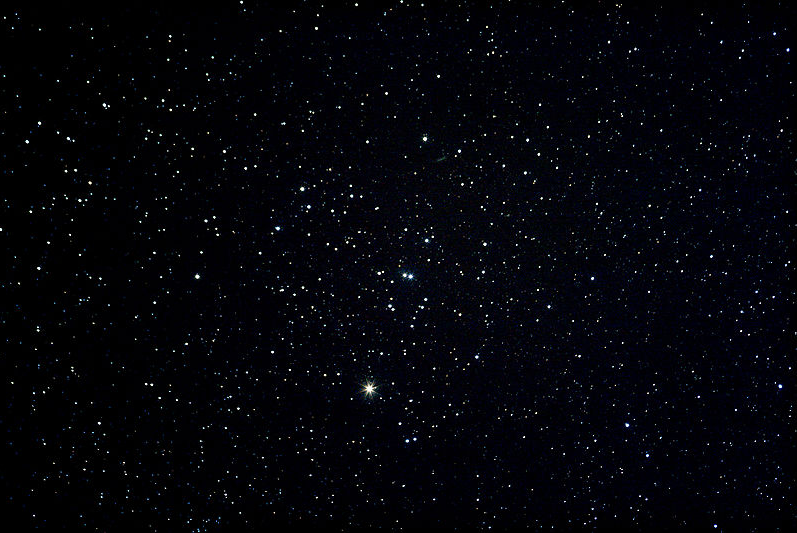
\includegraphics[width=.23\textwidth, height = 2.5 cm]{imagenes/introduction/hyades_int.png}
\includegraphics[width=.23\textwidth, height = 2.5 cm]{imagenes/introduction/coma_cluster.jpg}
\label{cm_beehive}
\caption{Left: Hyades open cluster.\footnote{\url{https://en.wikipedia.org/wiki/File:Coma.jpg}} Right: Coma open cluster.\footnote{\url{https://en.wikipedia.org/wiki/File:M45-_Hyades_(star_cluster).jpg}}}
\end{figure}
They are important to study because can be used to understand the star formation and evolution, structure, rotation curve and scale distances of the Milky Way. 
\end{minipage}
\end{frame}

\subsection{Motivation} 
\begin{frame}
\frametitle{Motivation}
\begin{minipage}{\textwidth}

\begin{figure}
    \centering
    \includegraphics[width=1\linewidth]{imagenes/introduction/coma_hyades_gaia_2018.png}
    \caption{Coma and Hyades selection made by \citep{Hyades_Gaia_2018}.}
    \label{fig:hyades_coma_gaia_2018}
\end{figure}
\end{minipage}
\end{frame}

\begin{frame}
\frametitle{Motivation}
\begin{minipage}{\textwidth}

\begin{figure}
    \centering
    \includegraphics[width=1\linewidth]{imagenes/introduction/cantat_gaudin_clusters.png}
\end{figure}
\end{minipage}
\end{frame}

\begin{frame}
\frametitle{Motivation}
\begin{minipage}{\textwidth}

\begin{figure}
    \centering
    \includegraphics[width=1\linewidth]{imagenes/introduction/emily_hunt_cluster.png}
\end{figure}
\end{minipage}
\end{frame}

\subsection{Scientific question and objectives}
\begin{frame}{Scientific Question}
\begin{minipage}\textwidth
    How to identify new physically open star clusters in the solar neighborhood using Gaia data, while avoiding the inclusion of spurious groupings that arise purely from statistical clustering?
\end{minipage}
    
\end{frame}

\subsection{Objectives}

\begin{frame}{Objectives}
\begin{minipage}\textwidth
     \begin{block}{General objective}
    Develop an automated pipeline for the reliable detection of 
    open clusters using Gaia data.
    \end{block}
    
    \vspace{0.4cm}
    
    \begin{columns}[T,onlytextwidth]
    
    \column{0.32\textwidth}
    \centering
    \textbf{1. Data Treatment}
    
    \vspace{0.2cm}
    
    Correct astrometric systematics and model observational uncertainties.
    
    \column{0.32\textwidth}
    \centering
    \textbf{2. Cluster Detection}
    
    \vspace{0.2cm}
    
    Apply \textbf{HDBSCAN} in high-dimensional astrometric space.
    
    \column{0.32\textwidth}
    \centering
    \textbf{3. Physical Validation}
    
    \vspace{0.2cm}
    
    Assess parallax coherence and consistency with stellar evolution.
    
    \end{columns}
\end{minipage}
    
\end{frame}

\begin{frame}{Gaia Data}
\begin{minipage}\textwidth
    Gaia appeared as a mission to make measurements 200 times more accurately than its antecessor Hipparcos. The spacecraft was launched on December 19 of 2013 and  it was orbiting in the second Lagrange point with a Lissajous-Type orbit at 1.5 million km with a period of 180 days until March 27 of 2025. 
    \begin{figure}
        \centering
        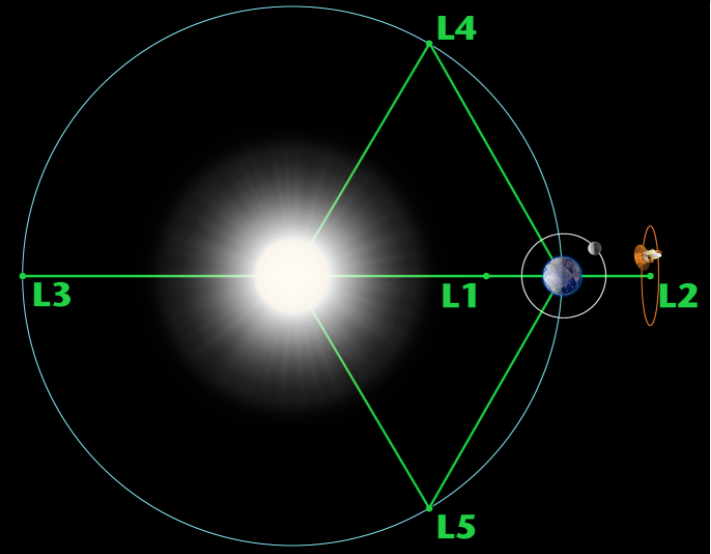
\includegraphics[scale=0.24]{imagenes/introduction/lagrange_points.png}
        \caption{Representation of the Lagrangian points for the system satellite, Sun and Earth.\footnote{\url{https://solarsystem.nasa.gov/resources/754/what-is-a-lagrange-point/}}}
        \label{fig:lagrange_gaia}
    \end{figure}
\end{minipage}
    
\end{frame}

\section{First approximation}

\begin{frame}
\frametitle{Exploration phase}
\begin{minipage}\textwidth
    Data was taken from the Gaia Archive, and it corresponds to Gaia Data Release 3, contents downloaded for this work are: \\
    \begin{itemize}
        \item Equatorial coordinates
        \item Proper motions
        \item Parallaxes
        \item $G$, $G_{RP}$ and $G_{BP}$ magnitudes
    \end{itemize}
    \vspace{0.5cm}
    
    Data were filtered by relative error on photometric, coordinates and proper motions variables, $RUWE<1.4$ and $visibility\_periods\_used>8$.
\end{minipage}
\end{frame}

\begin{frame}
\frametitle{Data filtering}
\begin{minipage}\textwidth
\textbf{Renormalized Unit Weight Error}:
\vspace{2mm}\\
(RUWE) is a key metric used to assess the quality of astrometric solutions. A value below 1.4 typically indicates a reliable fit, while higher values suggest potential issues, such as unresolved binary stars or poor data quality \cite{lindegren2021}.\\
    
\textbf{Visibility periods used}:
\vspace{2mm}\\
It represents distinct time intervals during which GAIA observes a source. A higher number of visibility periods indicates better coverage and more reliable data \cite{lindegren2018}.
\end{minipage}
\end{frame}

\begin{frame}{Gaia Data}
    There are two datasets centered in the coordinates:
    \begin{equation}
        (\alpha,\delta)_{hyades} = (66, 15)\;deg,
    \end{equation}
    \begin{equation}
        (\alpha,\delta)_{coma} = (193, 27)\;deg,
    \end{equation}
    
    with a radius of 40\;deg, as according to \cite{perryman} the Hyades OC is spreaded over $25\;deg$ in the sky.\\
    \vspace{5 mm}
    For stars brighter than 15 magnitudes, it has an accuracy on its measurements of $24\;\mu as$.
    Also, it has an accuracy over proper motions of about $1\;mas\;yr^{-1}.$
\end{frame}

\subsection{Members selection}

\subsubsection{Clustering Models}
\begin{frame}{Density-based spatial clustering of applications with noise}
\begin{minipage}\textwidth
    DBSCAN (Density-based spatial clustering of applications with noise) uses two hyperparameters $\epsilon$ and minimum number of points $minPts$ to classify the data points in three types \citep{ester1996,ester2017}:
    \begin{itemize}
        \item Central point
        \item Border point
        \item Outliers
    \end{itemize}
     \begin{figure}
     \centering
     
\includegraphics[scale=0.15]{imagenes/introduction/dbscan.png}
     \caption{DBSCAN description, image taken from \cite{ester2017}.}
     \label{fig:my_label}
 \end{figure}
\end{minipage}
\end{frame}

\begin{frame}
\frametitle{Feature Space for Clustering Analysis}
\begin{minipage}{\textwidth}

The clustering was performed in a multidimensional space defined by:
\begin{itemize}
    \item $\alpha$: Right Ascension (equatorial coordinate)
    \item $\delta$: Declination (equatorial coordinate)
    \item $\varpi$: Parallax
    \item $\mu_{\alpha^\ast}$: Proper motion in Right Ascension
    \item $\mu_{\delta}$: Proper motion in Declination
\end{itemize}

\end{minipage}
\end{frame} 

\begin{frame}
\frametitle{Standard cluster membership}
\begin{minipage}{\textwidth}

Initially with a unique selection of parameters we had the following results.

\begin{figure}[htp]
\begin{minipage}[b]{0.49\linewidth
}
    \centering
    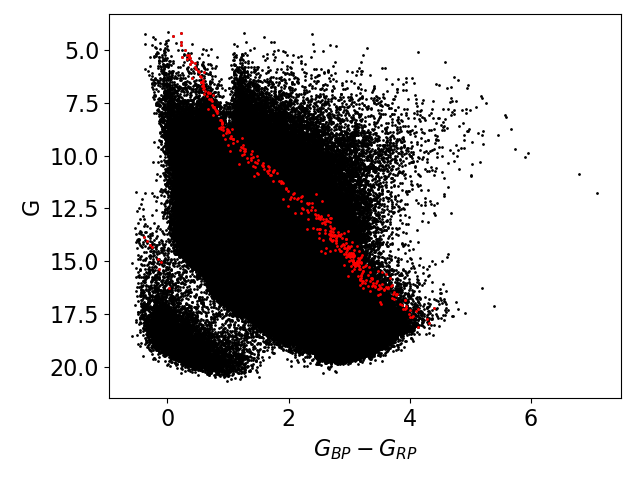
\includegraphics[width = \textwidth]{imagenes/res5/magnitude_5d.png}
\end{minipage}
\begin{minipage}[b]{0.49\linewidth}
    \centering
    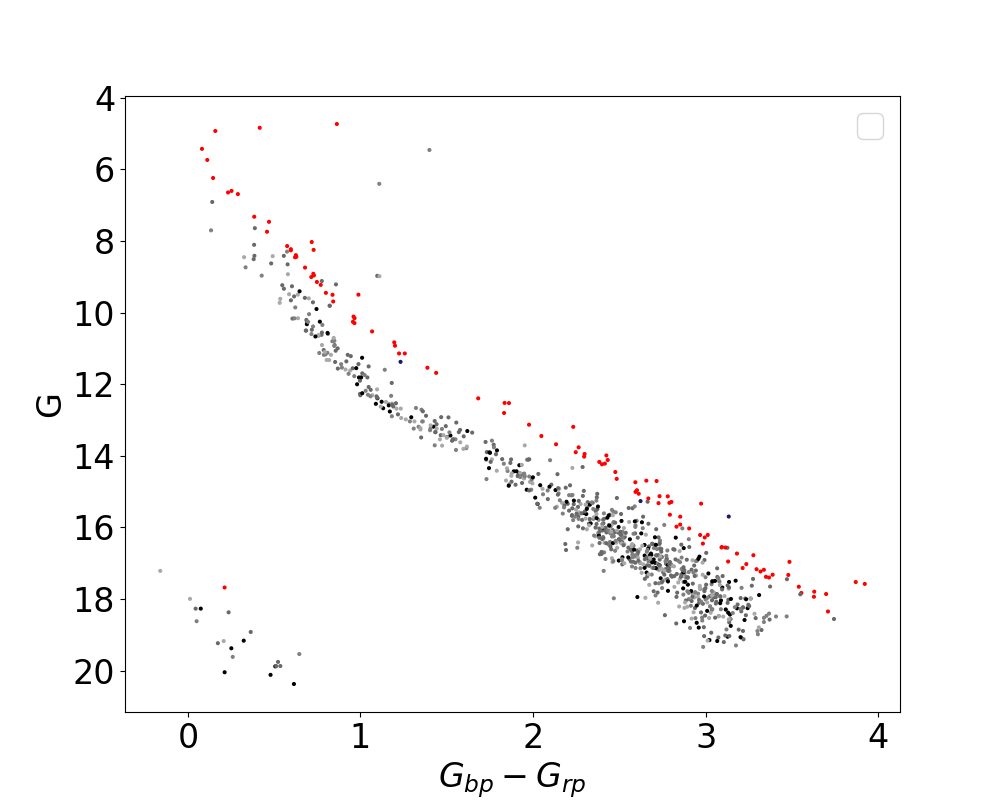
\includegraphics[width = \textwidth]{imagenes/res5/coma_selection.png}
\end{minipage}
    \caption{Left: 1098 Hyades members selected, Right: 937 Coma members selected.}
\label{fig:enter-label}
\end{figure} 

\end{minipage}
\end{frame} 

\begin{frame}
\frametitle{Spurious Cluster}
\begin{minipage}{\textwidth}

Using a unique selection of hyperparameters, some groupings were found, but they did not belong to any real cluster.

\begin{figure}[htp]
\begin{minipage}[b]{0.49\linewidth
}
    \centering
    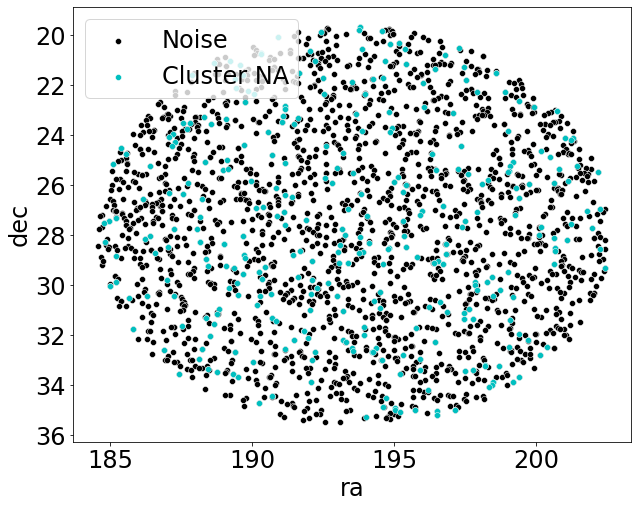
\includegraphics[width = \textwidth]{imagenes/res5/sp_coords.png}
\end{minipage}
\begin{minipage}[b]{0.445\linewidth}
    \centering
    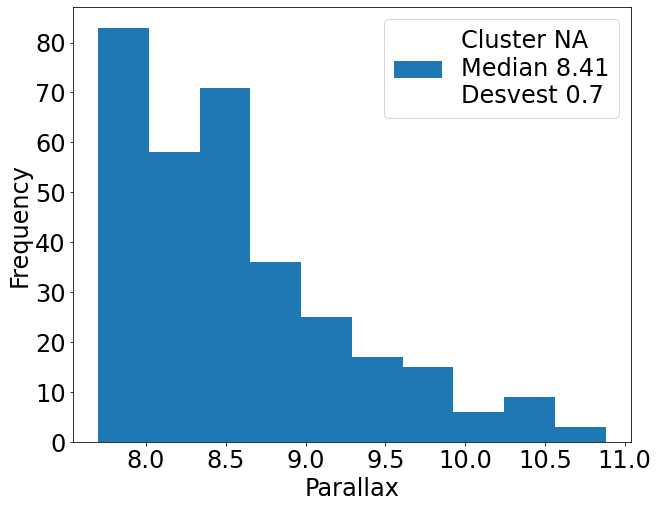
\includegraphics[width = \textwidth]{imagenes/res5/sp_parallax.png}
\end{minipage}
    \caption{Left: Unknown group in equatorial coordinates, Right: Parallax distribution for unknown group.}
\label{fig:enter-label}
\end{figure} 

\end{minipage}
\end{frame} 

\begin{frame}
\frametitle{Complement to DBSCAN}
\begin{minipage}{\textwidth}
We apply DBSCAN around 4 centers and with radii to capture different densities at the boundaries. Also, we apply a grid of posible epsilon and minPts to search clusters members.   

\begin{figure}[htp]
\begin{minipage}[b]{0.49\linewidth
}
    \centering
    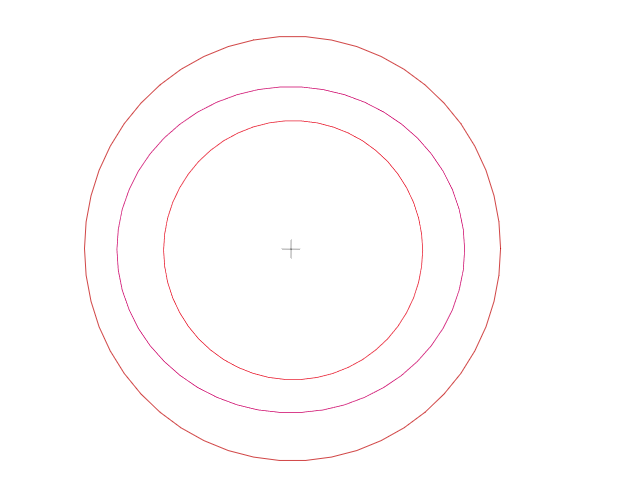
\includegraphics[width = \textwidth]{imagenes/dbscan/inicial_busqueda.png}
\end{minipage}
\begin{minipage}[b]{0.49\linewidth}
    \centering
    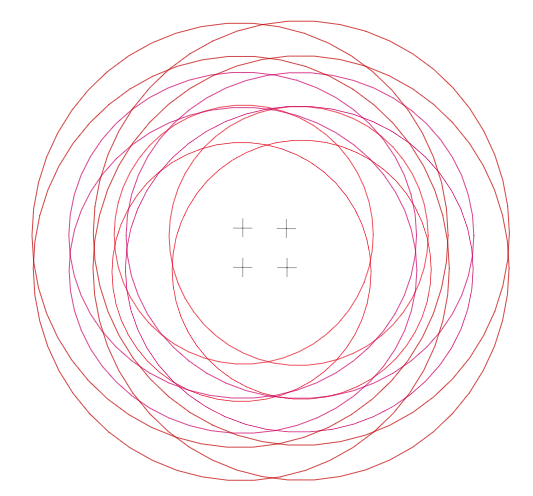
\includegraphics[width = \textwidth]{imagenes/dbscan/busqueda_total.png}
\end{minipage}
    \caption{Description of the method to apply DBSCAN.}
\end{figure}
\end{minipage}
\end{frame}

\begin{frame}{Membership Probability}
    \begin{minipage}\textwidth
    Each light source will, after a specific number of iterations, either belong or not to a cluster, providing us with a membership probability. In this way, we can select those sources with a higher probability. 
    \begin{figure}[htp]
\begin{minipage}[b]{0.49\linewidth
}
    \centering
    \includegraphics[width = \textwidth]{imagenes/res5/hyades_selection_prob.png}
\end{minipage}
\begin{minipage}[b]{0.49\linewidth}
    \centering
    \includegraphics[width = \textwidth]{imagenes/res5/coma_selection_prob.png}
\end{minipage}
    \caption{CM diagram for selecting members based on probability. Left: Hyades, right: Coma.}
\label{fig:prob_2_selection}
\end{figure} 
    \end{minipage}
\end{frame}

\subsection{First approximation results}

\begin{frame}{DBSCAN to assign membership}
\begin{minipage}\textwidth
    This new method has been used to find members to Hyades and Coma OC'S. These are the results:
\begin{figure}[htp]
\begin{minipage}[b]{0.49\linewidth
}
    \centering
    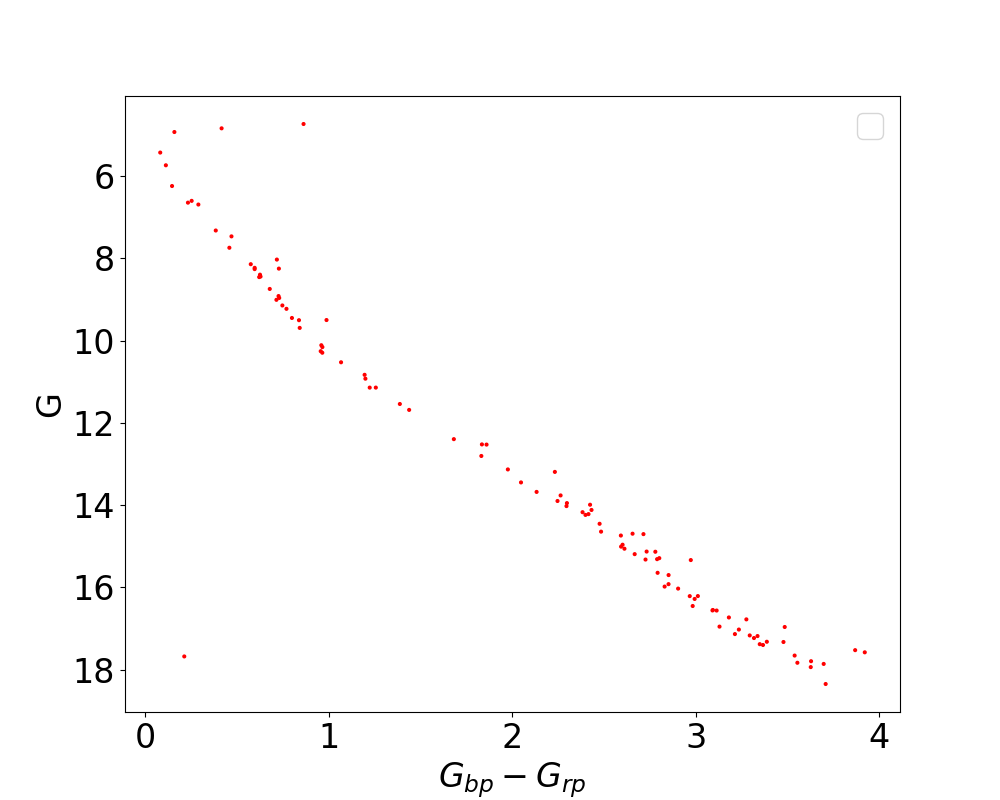
\includegraphics[width = \textwidth]{imagenes/res5/coma_magnitude2.png}
\end{minipage}
\begin{minipage}[b]{0.49\linewidth}
    \centering
    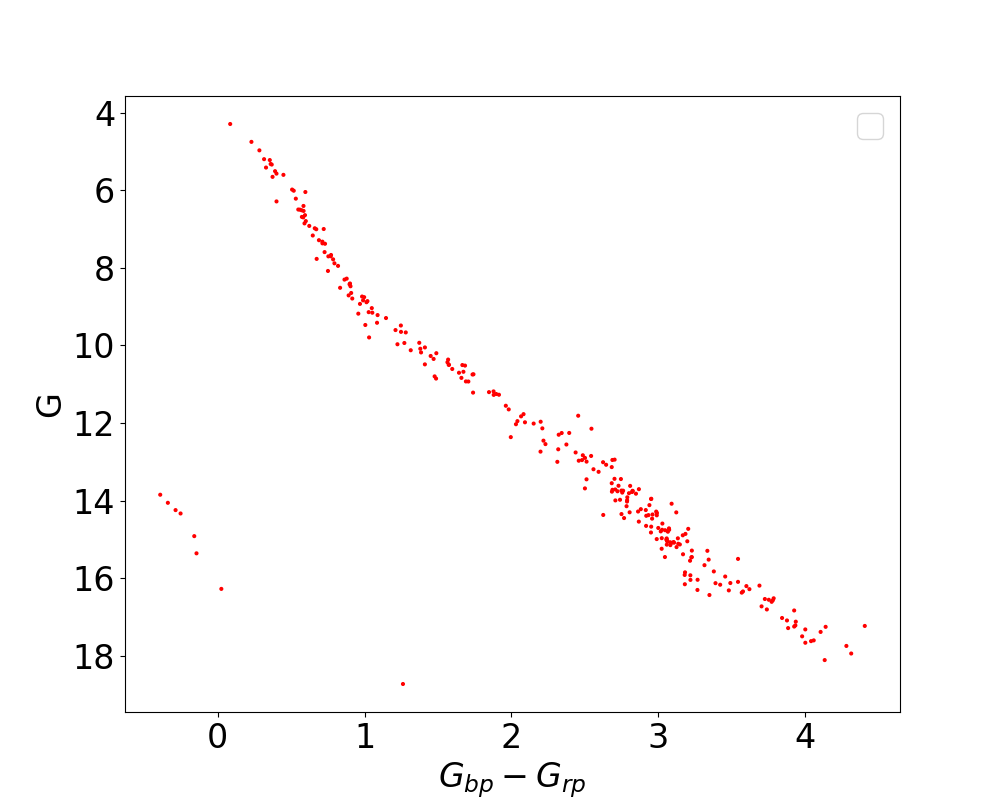
\includegraphics[width = \textwidth]{imagenes/res5/hyades_magnitude2.png}
\end{minipage}
    \caption{Left: Coma CM diagram (107 members). Righ: Hyades CM diagram. Membership results with the methodology shown (283 members).}
\end{figure}
    
\end{minipage}
x   \end{frame}

\section{Methodology}
\begin{frame}{Second Approach: 100 pc volume}
In this Second stage, we aim to recover well-known open clusters 
within the first 100 pc around the Sun.

\vspace{0.4cm}

\begin{itemize}
    \item \textbf{High completeness:} Gaia provides a volume-limited sample with $\sim 94\%$ completeness for parallax relative errors $< 10\%$ \citep{alberino2026newaxionboundsderived}.
    
    \item \textbf{Low contamination:} The Gaia nearby star catalog shows only $\sim 0.1\%$ contamination from false positives \citep{Lutsenko_2025}.
    
    \item \textbf{Uniform sampling:} Detection efficiency is high and homogeneous 
    across most of the 100 pc volume \citep{wang2026}.
    
    \item \textbf{Well-characterized benchmark region:} Contains the best-known open clusters (e.g., Hyades, Coma Berenices), ideal for validation.
\end{itemize}

\end{frame}

\begin{frame}{Hierarchical density-based spatial clustering of applications with noise}
\begin{minipage}\textwidth
HDBSCAN works by creating a tree of
clusters, then simplifying it to retain only
the most stable clusters.
By analyzing density variations, HDBSCAN
can handle noise better and find clusters in
datasets where density changes across
regions.
\begin{figure}
     \centering
     \includegraphics[scale=0.25]{imagenes/introduction/hdbscan_Example.png}
     \caption{HDBSCAN example (McInnes et al, 2016).}
     \label{fig:hdbsacn_dendogram}
 \end{figure}
\end{minipage}
\end{frame}

\subsection{Hyperparameters}

\begin{frame}{Hyperparameter Selection}
In order to obtain just 5 clusters, the $min\_cluster\_size$ is set to 200; however as in literature Coma sometimes tends to have fewer members than 200 hundred and we want to find new clusters, this parameter was set in 60 where we expect to have at least 20 clusters.
\begin{minipage}\textwidth
\begin{figure}
    \centering
    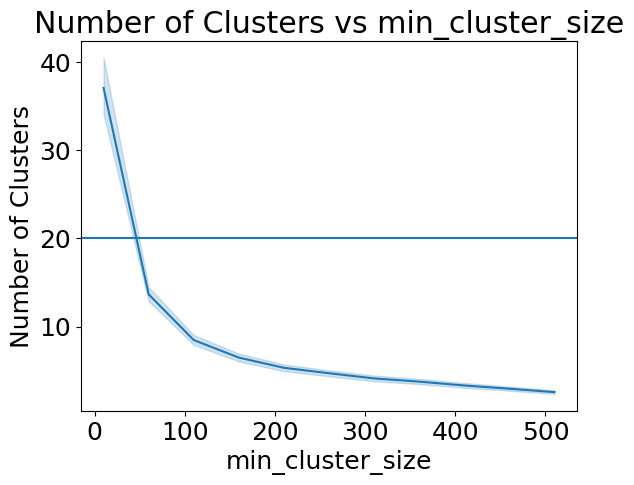
\includegraphics[width=0.5\linewidth]{imagenes/metodologia/min_cluster_size.png}
    \caption{$min\_cluster\_size$ graph for hyperparameter selection}
    \label{fig:min_cluster_size}
\end{figure}
    
\end{minipage}
\end{frame}

\begin{frame}{HDBSCAN to assign membership}
\begin{minipage}\textwidth
\begin{figure}
    \centering
    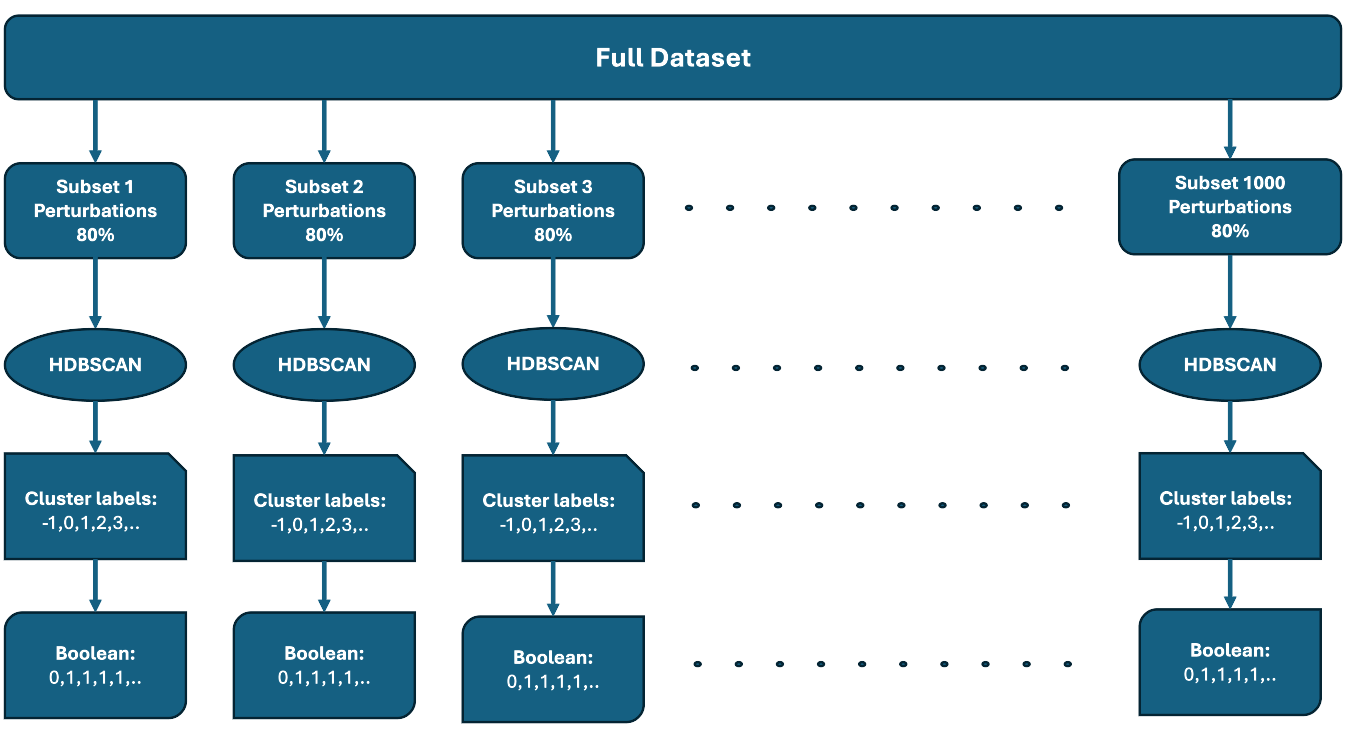
\includegraphics[width=1\linewidth]{imagenes/metodologia/metodologia_1.png}
    \caption{Methodology bootstrapping}
    \label{fig:method_part_1}
\end{figure}
    
\end{minipage}
\end{frame}

\begin{frame}{HDBSCAN to assign membership}
\begin{minipage}\textwidth
\begin{figure}
    \centering
    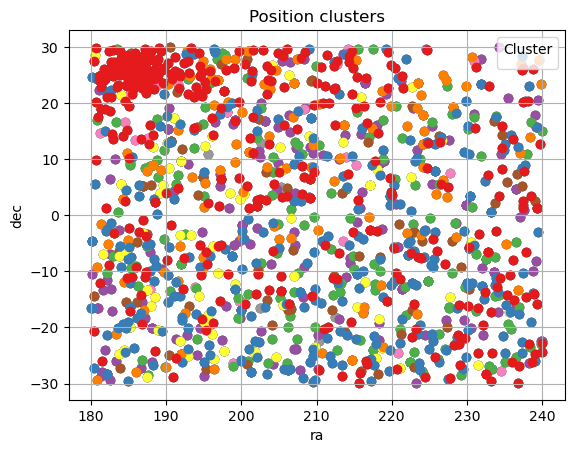
\includegraphics[width=0.5\linewidth]{imagenes/metodologia/coordinates_example.png}
    \caption{Coordinates example of $10^{th}$ iteration}
    \label{fig:coordinate_iteration}
\end{figure}
    
\end{minipage}
\end{frame}

\begin{frame}{HDBSCAN to assign membership}
\begin{minipage}\textwidth
\begin{figure}
    \centering
    
\includegraphics[width=0.5\linewidth]{imagenes/metodologia/example_pm.png}
    \caption{PM example of $10^{th}$ iteration}
    \label{fig:coordinate_iteration}
\end{figure}
    
\end{minipage}
\end{frame}

\begin{frame}{HDBSCAN to assign membership}
\begin{minipage}\textwidth
\begin{figure}
    \centering
    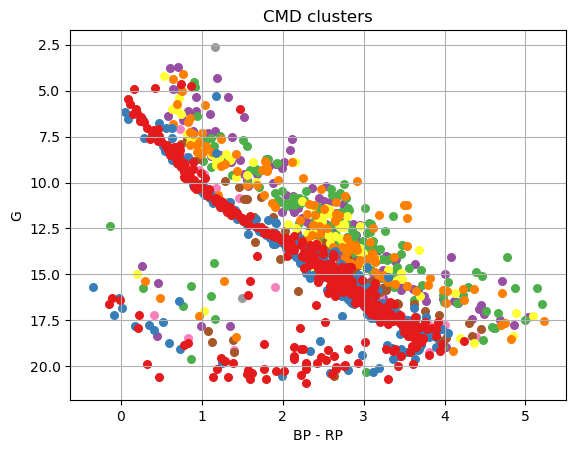
\includegraphics[width=0.5\linewidth]{imagenes/metodologia/cmd_example.png}
    \caption{CMD example of $10^{th}$ iteration}
    \label{fig:cmd_iteration}
\end{figure}
    
\end{minipage}
\end{frame}

\subsection{Metrics for selection}
\begin{frame}{Metrics}
\begin{minipage}\textwidth
\textbf{Presence in samples:}
This represents the number of times the star appeared in any cluster.
\begin{equation}
\Delta_{\text{presence}}(i) = \frac{\#(\text{samples where star } i \text{ is clustered})}{M},
\label{eq:frequency_metric}
\end{equation}
where $M$ is the number of iteratons where the $i$ star is present.\\
\vspace{1cm}

\textbf{ Silhouette Coefficient:}
It is a metric to evaluate clustering quality.

\begin{equation}
    Silhouette Coefficient: \frac{b - a}{ max(a, b)},
\label{eq:profile_silhouette}
\end{equation}

where $a$ is the average distance to points in the same cluster, and $b$ is the average distance to points in the nearest neighboring cluster. Values range from $-1$ (poor clustering) to $1$ (good clustering).
    
\end{minipage}
\end{frame}

\section{Preliminary Results}

\begin{frame}{Initial Dataset}
At the beginning the dataset has 398.944 registers.
\begin{minipage}\textwidth
\begin{figure}
    \centering
    
\includegraphics[width=0.8\linewidth]{figures/data_initial.png}
    \caption{Distribution of the stars downloaded from Gaia DR3.}
    \label{fig:galactic_preresult_method}
\end{figure}
    
\end{minipage}
\end{frame}

\begin{frame}{Data cleaning}
From bootstrapping with perturbation ensemble, we retained 10,916 stars ($2.2\%$ of the dataset) that were grouped at least once, filtering out those with extreme uncertainties to prevent contamination.
\begin{minipage}\textwidth
\begin{figure}
    \centering
    
\includegraphics[width=0.8\linewidth]{figures/data_process.png}
    \caption{Distribution of the stars retained after the bootstrapping process in Galactic coordinates. Only stars identified as members of a stellar grouping are shown.}
    \label{fig:galactic_result_method}
\end{figure}
    
\end{minipage}
\end{frame}

\begin{frame}{Top performing clusters- Hyades and Coma Berenices}
\begin{minipage}\textwidth
We identified a total of 57 distinct stellar groupings meeting our membership criterion. At the extreme, six clusters
emerged as statistically and physically superior to the remaining population according to the
joint evaluation of these metrics.
\begin{figure}
    \centering
    \begin{minipage}{0.48\textwidth}
        \centering
        
\includegraphics[width=1\linewidth]{figures/diagrama_cm_hyades.png}
    \end{minipage}
    \hfill
    \begin{minipage}{0.48\textwidth}
        \centering
        
\includegraphics[width=1\linewidth]{figures/diagrama_cm_coma.png}
    \end{minipage}
\end{figure}

    
\end{minipage}
\end{frame}
\subsection{Top performing clusters}
\begin{frame}{CM diagram}

\begin{minipage}\textwidth
The color-magnitude diagrams of the six detected clusters presented in the Figure reveal substantial diversity in stellar population structure and sequence definition quality.
\begin{figure}
    \centering

    % Primera fila
    \includegraphics[width=0.3\textwidth]{figures/diagrama_cluster_fidelity_8 Hyades.png}
    \hfill
    \includegraphics[width=0.3\textwidth]{figures/diagrama_cluster_fidelity_7 Coma Berenices.png}
    \hfill
    \includegraphics[width=0.3\textwidth]{figures/diagrama_cluster_fidelity_4.png}

    \vspace{0.3cm}

    % Segunda fila
    
\includegraphics[width=0.3\textwidth]{figures/diagrama_cluster_fidelity_13.png}
    \hfill
    
\includegraphics[width=0.3\textwidth]{figures/diagrama_cluster_fidelity_112.png}
    \hfill
    
\includegraphics[width=0.3\textwidth]{figures/diagrama_cluster_fidelity_16.png}
\end{figure}
\end{minipage}
\end{frame}

\begin{frame}{Parallax Histogram}

\begin{minipage}\textwidth
The parallax distributions for all six clusters are presented in Figure, organized in panels
corresponding to each detected grouping.
\begin{figure}[H]
    \centering

    % Primera fila
    
\includegraphics[width=0.3\textwidth]{figures/parallax_histogram_8 Hyades.png}
    \hfill
    
\includegraphics[width=0.3\textwidth]{figures/parallax_histogram_7 Coma Berenices.png}
    \hfill
    
\includegraphics[width=0.3\textwidth]{figures/parallax_histogram_4.png}

    \vspace{0.3cm}

    % Segunda fila
    
\includegraphics[width=0.3\textwidth]{figures/parallax_histogram_13.png}
    \hfill
    
\includegraphics[width=0.3\textwidth]{figures/parallax_histogram_112.png}
    \hfill
    
\includegraphics[width=0.3\textwidth]{figures/parallax_histogram_16.png}
\end{figure}
\end{minipage}
\end{frame}

\begin{frame}{Performance metrics}

\begin{minipage}\textwidth
The performance of each grouping according
to the adopted metrics is summarized in the following table.
\begin{table}
\centering
\small
\begin{tabular}{rrrrr}
\hline
ID cluster & Members & Silhouette & Effective Radius ($pc$) & Probability \\
\hline
8 (Hyades) & 476 & 0.648 & 4.98  & 0.795 \\
7 (Coma) & 248 & 0.523 & 10.06 & 0.789 \\
112 & 192 & 0.479 & 12.75 & 0.739 \\
4 & 76  & 0.170 & 10.45 & 0.704 \\
13 & 183 & 0.162 & 11.97 & 0.615 \\
16 & 215 & 0.683 & 12.05 & 0.463 \\
\hline
\end{tabular}
\end{table}
\end{minipage}
\end{frame}

\subsection{Clusters rejected}
\begin{frame}{CM diagram}

\begin{minipage}\textwidth
The color-magnitude diagrams of an example of six detected clusters presented in the Figure reveal different sequence definition some of them with a poor quality.
\begin{figure}
    \centering

    % Primera fila
    
\includegraphics[width=0.3\textwidth]{figures/diagrama_cluster_fidelity_116.png}
    \hfill
    \includegraphics[width=0.3\textwidth]{figures/diagrama_cluster_fidelity_90.png}
    \hfill
    
\includegraphics[width=0.3\textwidth]{figures/diagrama_cluster_fidelity_50.png}

    \vspace{0.3cm}

    % Segunda fila
    
\includegraphics[width=0.3\textwidth]{figures/diagrama_cluster_fidelity_80.png}
    \hfill
    \includegraphics[width=0.3\textwidth]{figures/diagrama_cluster_fidelity_415.png}
    \hfill
    
\includegraphics[width=0.3\textwidth]{figures/diagrama_cluster_fidelity_100.png}
\end{figure}
\end{minipage}
\end{frame}

\begin{frame}{Parallax Histogram}

\begin{minipage}\textwidth
The parallax distributions for the cluster examples are presented in Figure, organized in panels
corresponding to each detected grouping.
\begin{figure}[H]
    \centering

    % Primera fila
    
\includegraphics[width=0.3\textwidth]{figures/parallax_histogram_116.png}
    \hfill
    
\includegraphics[width=0.3\textwidth]{figures/parallax_histogram_90.png}
    \hfill
    
\includegraphics[width=0.3\textwidth]{figures/parallax_histogram_50.png}

    \vspace{0.3cm}

    % Segunda fila
    
\includegraphics[width=0.3\textwidth]{figures/parallax_histogram_80.png}
    \hfill
    
\includegraphics[width=0.3\textwidth]{figures/parallax_histogram_415.png}
    \hfill
    
\includegraphics[width=0.3\textwidth]{figures/parallax_histogram_100.png}
\end{figure}
\end{minipage}
\end{frame}

\subsection{Comparison with previous work}
\begin{frame}{Comparison with Previous Work}

\begin{minipage}\textwidth
Given the catalogue reported by \citep{hunt2023}, only four open clusters fall within the region of parameter space explored in this work and can therefore be directly compared with our detections.
\begin{itemize}
    \item Melotte 25 (Hyades) 
    \item Melotte 111 (Coma Berenices)
    \item HSC 396
    \item HSC 759
\end{itemize}
\end{minipage}
\end{frame}

\begin{frame}{Validation with known benchmark clusters}

\begin{minipage}\textwidth
For the first two cases, the results show good agreement with the literature. These correspond to the well-known benchmark open clusters:

\begin{figure}
    \centering
    \begin{minipage}{0.48\textwidth}
        \centering
        
\includegraphics[width=1\linewidth]{figures/comparacion_hyades.png}
    \end{minipage}
    \hfill
    \begin{minipage}{0.48\textwidth}
        \centering
        
\includegraphics[width=1\linewidth]{figures/comparacion_coma.png}
    \end{minipage}
\end{figure}


\end{minipage}
\end{frame}

\begin{frame}{Validation for HSC}

\begin{minipage}\textwidth
For these two Presence in Sample is significantly low.
As a consequence, their members are not sufficiently populated in our dataset and are embedded within the noise.

\begin{figure}
    \centering
    \begin{minipage}{0.48\textwidth}
        \centering
        
\includegraphics[width=1\linewidth]{figures/proportion_clusterings_HSC.png}
    \end{minipage}
    \hfill
    \begin{minipage}{0.48\textwidth}
        \centering
        
\includegraphics[width=1\linewidth]{figures/histogram_parallax_HSC.png}
    \end{minipage}
\end{figure}


\end{minipage}
\end{frame}

\begin{frame}{Cluster dispersion}

\begin{minipage}\textwidth
One way to assess whether a stellar overdensity corresponds to a real cluster is to quantify how spatially concentrated it is. For this purpose, we measured the radius of the structures. The results are summarized in the following table.

\begin{table}
\centering
\small
\begin{tabular}{rrrrr}
\hline
Cluster & Radius Median (pc) & Radius std (pc) \\
\hline
Melotte 25 / 8  & 6.00 & 6.41 \\
Melotte 111 / 7 & 12.18 & 10.21 \\
HSC 396 & 25.44 & 17.67  \\
HSC 759 & 18.07 & 12.47  \\
4    & 10.45 & 3.50 \\
13 (Andes 2)  & 11.97 & 4.27 \\
16 (Andes 1)   & 12.05 & 5.06 \\
112  & 12.75 & 4.89 \\
\hline
\end{tabular}
\end{table}

\end{minipage}
\end{frame}

\section{Conclusions}

\begin{frame}{Conclusions}
\begin{minipage}\textwidth
\begin{itemize}
    \item We have presented a comprehensive, end-to-end methodology for the automated detection and statistical validation of open clusters in large astrometric surveys.\\
    \item When applied to Gaia DR3 data, both at distances smaller and beyond than 100 parsecs, this methodology produces a comprehensive and statistically validated catalog of open clusters.
    \item The systematic application of the methodology developed here to these forthcoming datasets will enable the detection and characterization of the open cluster population across the Milky
Way.
\end{itemize}
\end{minipage}
\end{frame}

\section{Tentative timeline}

\begin{frame}{Tentative Timeline I}
\small
\renewcommand{\arraystretch}{1.25}

\begin{tabularx}{\textwidth}{p{2.4cm}X X}
\toprule
\textbf{Period} & \textbf{Objectives} & \textbf{Activities} \\
\midrule

2026-19 &
Complete the first stage of the research internship. &
Research internship; writing of Paper 1. \\

2026-20 (7th) &
Refine the non-member selection method and evaluate kinematic validation methods. &
Finalize Paper 1; continue thesis writing. \\

2027-10 (8th) &
Evaluate the impact of the method and compare results with the literature. &
Continue writing the doctoral thesis. \\

\bottomrule
\end{tabularx}

\end{frame}
\begin{frame}{Tentative Timeline II}
\small
\renewcommand{\arraystretch}{1.25}

\begin{tabularx}{\textwidth}{p{2.4cm}X X}
\toprule
\textbf{Period} & \textbf{Objectives} & \textbf{Activities} \\
\midrule

2027-19 &
Complete the final stage of the research internship. &
Research internship; writing of Paper 2. \\

2027-20 (9th) &
Apply the developed procedure to Gaia DR4 data. &
Apply the method to Gaia DR4; continue thesis writing; finalize Paper 2. \\

2028-10 (10th) &
Finalize the doctoral research and prepare the defense. &
Finalize thesis document; prepare dissertation materials. \\

\bottomrule
\end{tabularx}

\end{frame}

\section{References}
\begin{frame}
 \frametitle{References}
 \tiny
    \bibliography{referencias.bib}
    \bibliographystyle{apalike}
\end{frame}

\begin{frame}
\begin{minipage}{\textwidth}
 \frametitle{Selection of hyperparameters}
 DBSCAN requires of two hyperparameters to be executed these are the radius $\epsilon$ and minimum number of points $minPts$ \citep{ester2017}.\\
 \vspace{-0.1cm}
 To select the minPts there is an equation given by \cite{ester1996} which is:
 \vspace{-0.1cm}
 \begin{equation}
     minPts = 2\times dimension
 \end{equation}
 
 Usually, the radius $\epsilon$ takes the same value of the elbow for a k-distance plot, as is shown in the Figure~\ref{fig:k_distance_plot}.
 \vspace{-0.3cm}
 \begin{figure}
    \centering
    
\includegraphics[scale=0.3]{imagenes/introduction/ejemplo_codo1.jpg}
    \vspace{-0.2cm}
    \caption{Example of a k-distance plot. Image taken from \cite{dbscan2019}.}
    \label{fig:k_distance_plot}
\end{figure}
 
\end{minipage}
\end{frame}

\begin{frame}
\begin{minipage}{\textwidth}
 \frametitle{Selecion of hyperparameters}

 However, the dataset has some peculiarities. For example, multiple densities:  

\begin{figure}[htp]
\begin{minipage}[b]{0.35\linewidth
}
    \centering
    \includegraphics[width = \textwidth]{imagenes/res5/epsilon_plot.png}
\end{minipage}
\begin{minipage}[b]{0.35\linewidth}
    \centering
    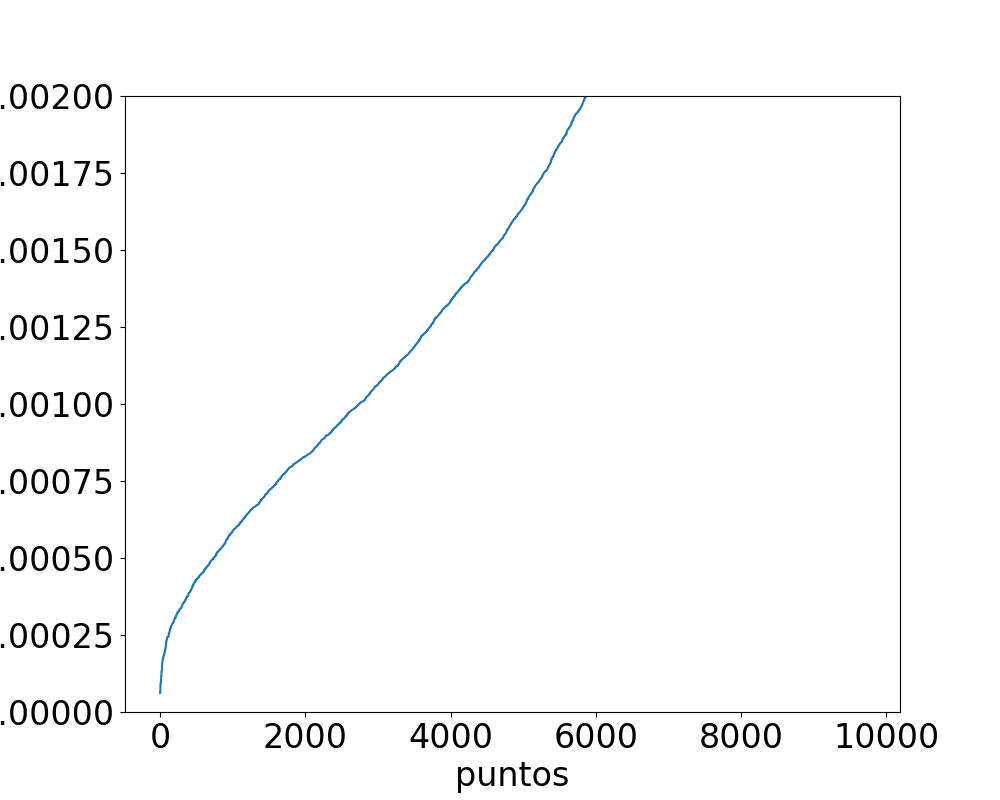
\includegraphics[width = \textwidth]{imagenes/res5/epsilon_plot_zoom.png}
\end{minipage}
    \caption{Left: Nearest neighbor distance plot, Right: Zoomed nearest neighbor distance plot.}
\label{fig:enter-label}
\end{figure} 
\end{minipage}
\end{frame}

\begin{frame}{Hyperparameter Selection}
Bootstrapping is computationally expensive, so we used this graph to determine the optimal number of iterations for efficiency.
\begin{minipage}\textwidth
\begin{figure}
    \centering
    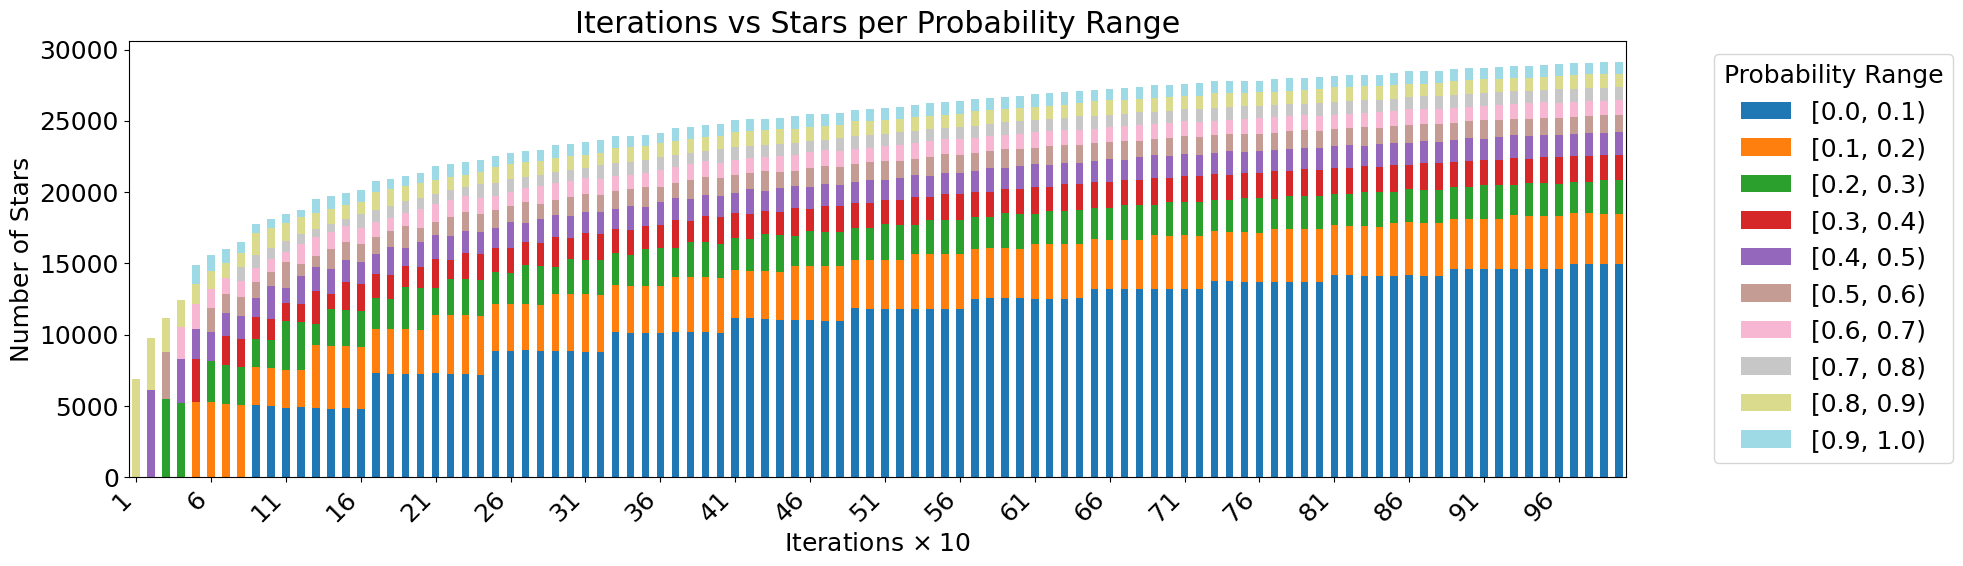
\includegraphics[width=1\linewidth]{imagenes/metodologia/iterations.png}
    \caption{Methodology bootstrapping}
    \label{fig:method_iterations}
\end{figure}
    
\end{minipage}
\end{frame}

\begin{frame}{Astrometric Fidelity}

\begin{block}{What is Fidelity?}
The \textbf{astrometric fidelity} parameter quantifies the reliability of Gaia astrometric solutions, helping to identify and remove spurious measurements \citep{Rybizki2021}.
\end{block}

\vspace{0.3cm}

\begin{itemize}
    \item Trained to distinguish good from bad astrometric solutions.
    
    \item Combines several Gaia quality indicators into a single reliability score.
    
    \item Useful to reduce contamination from sources with unreliable parallaxes or proper motions.
    
    \item Particularly important in cluster searches, where spurious astrometry can mimic false stellar overdensities.
\end{itemize}

\vspace{0.2cm}

\centering
\textit{We apply this criterion to ensure that detected structures are not driven by unreliable Gaia solutions.}

\end{frame}

\begin{frame}{Hyperparameter Selection}
The $min\_samples$ hyperparameter was kept at default, as increasing it reduced the number of clusters found below expectations \citep{CantatGaudin2020}.
\begin{minipage}\textwidth
\begin{figure}
    \centering
    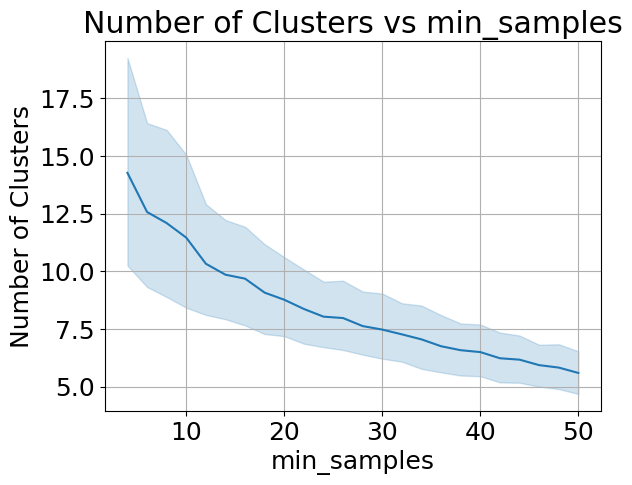
\includegraphics[width=0.5\linewidth]{imagenes/metodologia/min_samples.png}
    \caption{$min\_samples$ graph for hyperparameter selection}
    \label{fig:method_min_samples}
\end{figure}
    
\end{minipage}
\end{frame}

\begin{frame}{Validation for HSC}

\begin{minipage}\textwidth
For the remaining two clusters HSC 759 and HSC 396, the CMD are in the Figure:

\begin{figure}
    \centering
    \begin{minipage}{0.8\textwidth}
        \centering
        
\includegraphics[width=1\linewidth]{figures/scatter_BP_RP_G_HSC.png}
    \end{minipage}
\end{figure}


\end{minipage}
\end{frame}

\end{document}